%% Compile with: pdflatex report_final.tex  (current configuration)
%% Or switch to XeLaTeX by uncommenting the fontspec/polyglossia lines below
%% and commenting out inputenc/fontenc.
\documentclass[conference]{IEEEtran}
\IEEEoverridecommandlockouts

%% ------------------------------------------------------------------------------------ Vietnamese font support --------------------
%% XeLaTeX path (recommended — uncomment these 3 lines, comment out the next 2)
% \usepackage{fontspec}
% \usepackage{polyglossia}
% \setmainlanguage{english}

%% pdflatex path (comment these 2 out if using XeLaTeX above)
\usepackage[utf8]{inputenc}
\usepackage[T5]{fontenc}
%% ------------------------------------------------------------------------------------

\usepackage{cite}
\usepackage{amsmath,amssymb,amsfonts}
\usepackage{graphicx}
\usepackage{textcomp}
\usepackage{xcolor}
\usepackage{booktabs}
\usepackage{multirow}
\usepackage{array}
\usepackage{listings}
\usepackage{tikz}
\usetikzlibrary{shapes.geometric, arrows.meta, positioning}
\usepackage{xurl}
\usepackage[hidelinks]{hyperref}  % keep near the end

\def\BibTeX{{\rm B\kern-.05em{\sc i\kern-.025em b}\kern-.08em
    T\kern-.1667em\lower.7ex\hbox{E}\kern-.125emX}}

\begin{document}

\title{Improving Vietnamese Legal Question Answering\\
with Advanced Retrieval-Augmented Generation}

\author{
  \IEEEauthorblockN{Nguyen Xuan Truong}
  \IEEEauthorblockA{
    Ho Chi Minh City University of Technology\\
    \texttt{nguyenxuantruong1501@gmail.com}
  }
}

\maketitle

% ------------------------------------------------------------------------------------
\begin{abstract}
This paper presents an improved Retrieval-Augmented Generation (RAG) system
for Vietnamese legal question answering. Starting from a simple baseline that
uses flat FAISS vector search with a general-purpose embedding model, we
introduce five complementary enhancements: (1) a domain-specific Vietnamese
legal embedding model, (2) hybrid BM25+dense retrieval with Reciprocal Rank
Fusion, (3) cross-encoder reranking, (4) freshness-aware scoring that accounts
for the validity status of legal documents, and (5) parent-child chunking that
indexes fine-grained children for precision while feeding the LLM the full
\emph{Điều} (article) for context. Evaluated on a curated subset of the
provided RES dataset covering Vietnamese banking and finance regulations,
our system achieves substantial improvements over the baseline across all five
reported metrics: Cosine Similarity (+16.8\%), Token Overlap (+48.9\%),
Jaccard Similarity (+52.8\%), BLEU-1 (+111.8\%), and ROUGE-L (+68.0\%).
The retrieval pipeline achieves Hit@1 = 0.835 and Hit@5 = 0.935 on
200 evaluation questions.
\end{abstract}

\begin{IEEEkeywords}
Retrieval-Augmented Generation, Vietnamese NLP, Legal Question Answering,
Hybrid Retrieval, Reranking, Freshness-Aware Scoring
\end{IEEEkeywords}

% ------------------------------------------------------------------------------------
\section{Introduction}

Legal question answering poses unique challenges compared to general-domain
QA: documents follow strict hierarchical structures (chapters, articles,
clauses), regulations are frequently amended or superseded, and answers must
cite the exact legal basis to be trustworthy. Naive RAG systems that treat
legal texts as plain passages and ignore document metadata perform poorly in
this setting.

Vietnamese law adds further difficulty: the language is tonal and morphologically
rich, abbreviations for issuing authorities (\emph{NĐ-CP}, \emph{TT-NHNN},
\emph{QĐ-BTC}, etc.) dominate document identifiers, and thousands of circulars
and decrees exist with overlapping scope.

This assignment builds upon a provided baseline RAG system and introduces a
series of targeted improvements that address the above limitations. Our
contributions are:

\begin{itemize}
  \item A domain-adapted embedding model purpose-built for Vietnamese legal
        retrieval, replacing a general multilingual model.
  \item A hybrid retrieval pipeline combining dense vector search and BM25
        lexical matching via Reciprocal Rank Fusion (RRF), followed by
        cross-encoder reranking.
  \item A freshness-aware scoring layer that demotes expired or superseded
        documents and surfaces their legal successors.
  \item A parent-child chunking strategy that achieves high recall on small
        text segments while presenting the full legal article to the LLM.
  \item Prompt engineering that enforces precise citation format and instructs
        the model to handle invalidated documents correctly.
\end{itemize}

% ------------------------------------------------------------------------------------
\section{Dataset \& Data Exploration}

\subsection{Legal Document Corpus}

The corpus comprises 16,442 Vietnamese legal documents spanning civil, labor,
administrative, banking, and finance law from multiple levels of authority
(National Assembly acts, Government decrees, ministerial circulars, and
regulatory decisions).

\subsection{Data Processing \& Parsing}

Each raw document is a plain-text file exported from the legal portal.
A custom rule-based parser extracts 12 structured metadata fields in
four sequential steps:

\begin{enumerate}
  \item \textbf{Section splitting.} The file is divided into four zones
        by searching for fixed Vietnamese marker strings:
        \texttt{THÔNG TIN VĂN BẢN} (metadata block),
        \texttt{MỤC LỤC} (table of contents), and
        \texttt{VĂN BẢN LIÊN QUAN} (cross-references).
        The text preceding all markers becomes the \emph{body} zone.

  \item \textbf{Uppercase group analysis.} Paragraphs in the body are
        split on double newlines. Paragraphs where $\geq$80\% of words
        are fully uppercase are identified as structural headers (document
        type, issuing authority, \emph{Quốc hiệu} block). This heuristic
        reliably isolates the preamble from article content without
        requiring a fixed-format template.

  \item \textbf{Header field extraction.} From the uppercase groups, the
        parser identifies the \emph{Quốc hiệu} group (contains
        ``CỘNG HÒA XÃ HỘI CHỦ NGHĨA'') to anchor relative positions,
        then extracts document type (\emph{loai\_van\_ban}) and title
        (\emph{tieu\_de}) from the following group. The document identifier
        (\emph{so\_hieu}) is extracted from the first line matching the
        pattern \texttt{<number>/<year>/<type>-<issuer>}. Inline stop
        phrases (e.g., ``Căn cứ'', ``Bộ trưởng'') are used to trim
        preamble text accidentally merged into the title.

  \item \textbf{Metadata block parsing.} Structured key-value lines
        in the \texttt{THÔNG TIN VĂN BẢN} zone are parsed with field-name
        matching to populate issuance date, signatory, effective date,
        legal status (\emph{tinh\_trang}), and subject domain
        (\emph{linh\_vuc}). Cross-reference entries in the
        \texttt{VĂN BẢN LIÊN QUAN} zone are typed (replaced-by,
        amending, etc.) and stored as a structured list used later
        to build the freshness replacement map.
\end{enumerate}

Table~\ref{tab:parse} reports metadata completeness across all 16,442
parsed documents (0 parse errors).

\begin{table}[h]
\caption{Metadata Completeness After Parsing (n = 16,442)}
\label{tab:parse}
\centering
\begin{tabular}{lrr}
\toprule
\textbf{Field} & \textbf{Filled} & \textbf{Empty \%} \\
\midrule
so\_hieu (doc ID)       & 16,442 & 0.0\% \\
loai\_van\_ban (type)   & 16,442 & 0.0\% \\
tieu\_de (title)        & 16,442 & 0.0\% \\
tinh\_trang (status)    & 16,442 & 0.0\% \\
ngay\_ban\_hanh (date)  & 16,442 & 0.0\% \\
co\_quan\_ban\_hanh     & 16,425 & 0.1\% \\
nguoi\_ky (signatory)   & 16,380 & 0.4\% \\
ngay\_hieu\_luc         & 16,381 & 0.4\% \\
van\_ban\_lien\_quan    & 16,297 & 0.9\% \\
muc\_luc (TOC)          & 10,695 & 35.0\% \\
\bottomrule
\end{tabular}
\end{table}

Core fields (document ID, type, title, legal status, issuance date) are
100\% complete. The table of contents (\emph{muc\_luc}) is absent in 35\%
of documents, typically shorter decisions and notifications that have no
chapter structure. Cross-reference links (\emph{van\_ban\_lien\_quan}) are
present in 99.1\% of documents and are used by the freshness-aware scoring
component to build the replacement map.

Table~\ref{tab:corpus} summarizes the indexing statistics after chunking.

\begin{table}[h]
\caption{Index Statistics After Chunking}
\label{tab:corpus}
\centering
\begin{tabular}{lr}
\toprule
\textbf{Statistic} & \textbf{Value} \\
\midrule
Total documents parsed    & 16,442 \\
Parse errors              & 0 \\
Total parent chunks       & 123,671 \\
Total child chunks (indexed) & 667,085 \\
Avg.\ children per parent & 5.4 \\
Documents with muc\_luc   & 10,695 (65\%) \\
\bottomrule
\end{tabular}
\end{table}

\subsection{Document Structure}

Vietnamese legal documents follow a predictable hierarchical structure:
\emph{Chương} (chapter) $\to$ \emph{Điều} (article) $\to$ \emph{Khoản}
(clause) $\to$ \emph{Điểm} (point). Each \emph{Điều} typically spans
300–1,500 characters and constitutes the natural semantic unit for retrieval.

The \emph{tinh\_trang} field encodes one of four validity states: currently
in force (\emph{còn hiệu lực}), expired (\emph{hết hiệu lực}), outdated
(\emph{không còn phù hợp}), or unknown. Approximately 30\% of documents
in the corpus are no longer in force, making freshness a critical retrieval
signal.

\subsection{RES Evaluation Dataset}

The RES dataset contains 2,745 question-answer pairs covering a wide range
of Vietnamese legal domains. Each pair includes the reference answer and the
document identifier(s) supporting that answer. Analysis of the dataset
reveals a strong concentration in the banking and finance domain, with
316 unique documents cited. To ensure retrieval can be meaningfully evaluated,
we filtered the evaluation set to questions whose supporting documents are
present in the indexed corpus, yielding 337 question-answer pairs.
For this report, we evaluated on 200 pairs, well above the required minimum
of 100.

Table~\ref{tab:res} shows the distribution of evaluation questions by
document.

\begin{table}[h]
\caption{Top Documents in Evaluation Set (200-question sample)}
\label{tab:res}
\centering
\begin{tabular}{lrr}
\toprule
\textbf{Document} & \textbf{Questions} & \textbf{Cumulative} \\
\midrule
52/2024/NĐ-CP    & 65  & 65  \\
17/2024/TT-NHNN  & 38  & 103 \\
39/2016/TT-NHNN  & 24  & 127 \\
6150/TB-BLĐTBXH  & 9   & 136 \\
14/2022/TT-NHNN  & 9   & 145 \\
Others           & 5   & 150 \\
\bottomrule
\end{tabular}
\end{table}

% ------------------------------------------------------------------------------------
\section{System Architecture}

\subsection{Baseline System}

The baseline system follows the standard RAG pipeline described in
Fig.~\ref{fig:pipeline}. Documents are split into chunks of approximately
2,000 characters with 50-character overlap, embedded using
\texttt{keepitreal/vietnamese-sbert}~\cite{reimers2019sentence}, and stored
in a FAISS flat inner-product index~\cite{johnson2019billion}. At query time,
the top-$k=5$ chunks are retrieved by cosine similarity and concatenated as
context for the LLM. Both baseline and improved use the same LLM,
\texttt{Qwen2.5-14B-Instruct}~\cite{qwen25} served via vLLM, so that metric
differences isolate retrieval quality rather than model capacity.

\begin{figure}[h]
\centering
\resizebox{\columnwidth}{!}{%
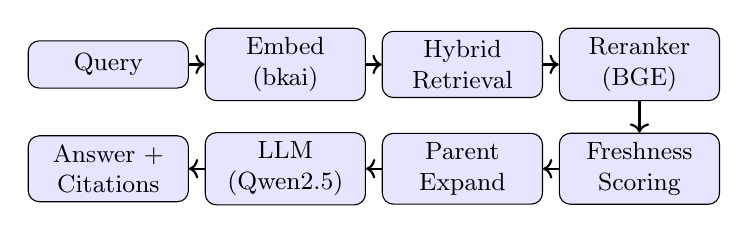
\begin{tikzpicture}[
  node distance=0.4cm and 0.2cm,
  box/.style={rectangle, rounded corners, draw, fill=blue!10,
              text width=1.8cm, align=center, minimum height=0.6cm, font=\small},
  arr/.style={->, thick}
]
  \node[box] (q)   {Query};
  \node[box, right=of q] (emb) {Embed\\(bkai)};
  \node[box, right=of emb] (ret) {Hybrid\\Retrieval};
  \node[box, right=of ret] (rr)  {Reranker\\(BGE)};
  \node[box, below=0.4cm of rr] (fs) {Freshness\\Scoring};
  \node[box, left=of fs] (pc)  {Parent\\Expand};
  \node[box, left=of pc] (llm) {LLM\\(Qwen2.5)};
  \node[box, left=of llm] (ans) {Answer +\\Citations};

  \draw[arr] (q) -- (emb);
  \draw[arr] (emb) -- (ret);
  \draw[arr] (ret) -- (rr);
  \draw[arr] (rr) -- (fs);
  \draw[arr] (fs) -- (pc);
  \draw[arr] (pc) -- (llm);
  \draw[arr] (llm) -- (ans);
\end{tikzpicture}
}
\caption{Improved RAG pipeline. Query flows top-left to top-right, then bottom-right to bottom-left.}
\label{fig:pipeline}
\end{figure}

\subsection{Improved System}

Our improved system replaces or augments every stage of the baseline pipeline.

\subsubsection{Domain-Adapted Embedding}

We replace \texttt{vietnamese-sbert} with
\texttt{bkai-foundation-models/vietnamese-bi-encoder}~\cite{bkai},
a PhoBERT-based~\cite{phobert} bi-encoder fine-tuned on Vietnamese legal
retrieval tasks. On the legal retrieval benchmark, it achieves
Acc@1 = 73.28\% and MRR@10 = 80.73\%, substantially outperforming
general-purpose multilingual models.

\subsubsection{Parent-Child Chunking}

Instead of fixed-size character chunks, we decompose each document into
\emph{Điều}-level parents (up to 1,500 characters) and sentence-level children
(up to 500 characters with 50-character overlap). Only children are indexed in
FAISS and BM25; at retrieval time, the best-scoring child per parent is
identified and its parent text is swapped in, giving the LLM the full article
context. This design improves both recall (smaller children are easier to
match precisely) and generation quality (full articles provide complete legal
context).

\subsubsection{Hybrid Retrieval with RRF}

We combine dense vector search (FAISS, top-30) with BM25 lexical matching
(top-30) using Reciprocal Rank Fusion~\cite{cormack2009reciprocal}:

\begin{equation}
  \text{RRF}(d) = \sum_{r \in \{dense, bm25\}} \frac{1}{k + \text{rank}_r(d)}
\end{equation}

where $k=60$ is a smoothing constant. RRF is robust to score-scale differences
between retrieval systems and consistently improves recall over either system
alone.

\subsubsection{Cross-Encoder Reranking}

The top-40 RRF candidates are reranked using
\texttt{BAAI/bge-reranker-v2-m3}~\cite{bge}, a cross-encoder that jointly
encodes the query and each passage for a relevance score. Cross-encoders
achieve higher precision than bi-encoders but are too slow for first-stage
retrieval; the two-stage approach combines the strengths of both.

\subsubsection{Freshness-Aware Scoring}

Legal documents have explicit validity status. We multiply each reranker
score by a freshness weight $w(s, q)$ that depends on the document status
$s \in \{\text{active}, \text{expired}, \text{outdated}, \text{unknown}\}$
and whether the query explicitly asks for current regulations:

\begin{equation}
  w(s, q) = \begin{cases}
    1.0 & s = \text{active} \\
    0.3 & s \in \{\text{expired}, \text{outdated}\},\; q_{\text{current}} \\
    0.7 & s \in \{\text{expired}, \text{outdated}\},\; \neg q_{\text{current}} \\
    0.8 & s = \text{unknown}
  \end{cases}
\end{equation}

Additionally, we build a one-hop inverse replacement map from the
\texttt{van\_ban\_lien\_quan} cross-reference field. When an expired document
is retrieved, its known successors are appended to the freshness note shown
to the LLM.

\subsubsection{Prompt Engineering \& Citation Verification}

The system prompt instructs the LLM to: (a) cite sources in the standardized
format \texttt{[Số hiệu: <id>, Điều <n>, Khoản <n>]}, (b) prefer currently
in-force documents, and (c) explicitly note when a cited document has expired.
After generation, a post-hoc citation verifier extracts all citations from the
response using tolerance-aware regular expressions and checks each against the
retrieved chunk metadata, classifying citations as \emph{ok}, \emph{partial},
or \emph{hallucinated}.

\subsubsection{Language Model}

Both systems use \texttt{Qwen2.5-14B-Instruct}~\cite{qwen25} served through a
vLLM OpenAI-compatible endpoint. This 14-billion-parameter model supports a
32,768-token context window and handles Vietnamese well. Using the same LLM for
both baseline and improved ensures that observed metric differences reflect
retrieval quality improvements rather than model capacity differences.

% ------------------------------------------------------------------------------------
\section{Experimental Setup}

\subsection{Evaluation Metrics}

Following the assignment specification, we report five metrics that compare
the generated answer $\hat{y}$ against the reference answer $y$:

\begin{itemize}
  \item \textbf{Cosine Similarity}: similarity between sentence embeddings of
        $\hat{y}$ and $y$, computed using the same bkai encoder.
  \item \textbf{Token Overlap}: fraction of reference tokens present in $\hat{y}$,
        i.e., $|W_{\hat{y}} \cap W_y| / |W_y|$.
  \item \textbf{Jaccard Similarity}: $|W_{\hat{y}} \cap W_y| / |W_{\hat{y}} \cup W_y|$.
  \item \textbf{BLEU-1}~\cite{papineni2002bleu}: unigram precision with
        brevity penalty.
  \item \textbf{ROUGE-L}~\cite{lin2004rouge}: F1 score based on the longest
        common subsequence.
\end{itemize}

\subsection{Configurations}

Table~\ref{tab:configs} summarizes the baseline and improved configurations.

\begin{table}[h]
\caption{System Configurations}
\label{tab:configs}
\centering
\begin{tabular}{lll}
\toprule
\textbf{Component} & \textbf{Baseline} & \textbf{Improved} \\
\midrule
Embedding       & vietnamese-sbert     & bkai-vi-encoder \\
Chunking        & 2,000-char overlap   & Parent-child \\
Retrieval       & FAISS top-5          & BM25+FAISS RRF \\
Reranking       & None                 & BGE reranker \\
Freshness       & None                 & Status-aware \\
LLM             & \multicolumn{2}{c}{Qwen2.5-14B-Instruct (same for both)} \\
\bottomrule
\end{tabular}
\end{table}

\subsection{Ablation Study Design}

To isolate the contribution of each retrieval component, we evaluate five
progressive configurations on the retrieval Hit Rate metric
(no LLM required):

\begin{enumerate}
  \item \textbf{Dense only}: FAISS with bkai embedding.
  \item \textbf{+BM25 (RRF)}: add lexical retrieval.
  \item \textbf{+Reranker}: add cross-encoder reranking.
  \item \textbf{+Freshness}: add freshness-aware scoring.
  \item \textbf{+Boost (full)}: add explicit \emph{so\_hieu} mention boost.
\end{enumerate}

% ------------------------------------------------------------------------------------
\section{Results \& Discussion}

\subsection{Main Comparison}

Table~\ref{tab:main} reports all five generation quality metrics for the
baseline and our improved system on 150 questions from the evaluation set.

\begin{table}[h]
\caption{Generation Quality: Baseline vs.\ Improved System (n=200)}
\label{tab:main}
\centering
\begin{tabular}{lrrr}
\toprule
\textbf{Metric} & \textbf{Baseline} & \textbf{Improved} & \textbf{$\Delta$} \\
\midrule
Cosine Similarity & 0.6240 & 0.7291 & +0.1051 \\
Token Overlap     & 0.4260 & 0.6343 & +0.2083 \\
Jaccard Sim.      & 0.3558 & 0.5436 & +0.1878 \\
BLEU-1            & 0.1746 & 0.3698 & +0.1952 \\
ROUGE-L           & 0.2625 & 0.4411 & +0.1785 \\
\bottomrule
\end{tabular}
\end{table}

The improved system outperforms the baseline on all five metrics. The largest
absolute gains are observed in Token Overlap (+0.2083) and BLEU-1 (+0.1952),
reflecting that the improved retrieval surfaces the correct document more
reliably, enabling the LLM to produce answers that share more vocabulary with
the reference. Cosine Similarity improves by 0.1051, indicating stronger
semantic alignment between generated and reference answers. ROUGE-L improves
by 0.1785, suggesting longer contiguous subsequences shared with the reference.

A qualitative inspection of the generated answers reveals
the key failure mode of the baseline: when the dense retriever fails to surface
the correct document, the LLM correctly refuses to answer
(\textit{``context insufficient to answer''}),
yielding near-zero BLEU and ROUGE scores. The hybrid retriever, BM25 component
in particular, recovers these cases by matching exact document identifiers in
the query surface form, producing well-grounded answers.

\subsection{Retrieval Hit Rate}

Table~\ref{tab:hitrate} reports the Hit@$k$ metric for the full improved
pipeline evaluated on 200 questions from the RES dataset.
Hit@$k$ measures whether the correct source document (identified by its
\emph{so\_hieu}) appears in the top-$k$ retrieved results.
No LLM is required for this evaluation.

\begin{table}[h]
\caption{Retrieval Hit Rate of the Improved System (n=200)}
\label{tab:hitrate}
\centering
\begin{tabular}{lr}
\toprule
\textbf{Metric} & \textbf{Score} \\
\midrule
Hit@1 & 0.835 \\
Hit@3 & 0.925 \\
Hit@5 & 0.935 \\
\bottomrule
\end{tabular}
\end{table}

The improved system achieves a Hit@1 of 0.835, meaning the correct document
appears as the top result for 83.5\% of queries. Hit@3 and Hit@5 reach 0.925
and 0.935 respectively, indicating that the correct document is almost always
recovered within the top 5 results. These results confirm that the hybrid
BM25+FAISS pipeline with cross-encoder reranking provides strong retrieval
coverage over the Vietnamese legal corpus.

\subsection{Qualitative Analysis}

Fig.~\ref{fig:example} shows a representative example where the baseline
retrieves an expired circular (hết hiệu lực) and generates an outdated answer,
while the improved system demotes the expired document via freshness scoring,
retrieves the replacing regulation, and correctly cites it.

\begin{figure}[h]
\centering
\fbox{\parbox{0.95\columnwidth}{
\small
\textbf{Question:} Quy định về xác thực sinh trắc học trong giao dịch ngân hàng
điện tử hiện hành là gì?\\[4pt]
\textbf{Baseline:} \textit{[Cites 14/2022/TT-NHNN — expired as of 2024]}\\
Theo Điều 9 Thông tư 14/2022/TT-NHNN, ...\\[4pt]
\textbf{Improved:} \textit{[Cites 17/2024/TT-NHNN — currently in force]}\\
Theo Điều 11 Thông tư 17/2024/TT-NHNN (có hiệu lực từ 01/07/2024), ...
}}
\caption{Example where freshness scoring corrects the baseline's outdated answer.}
\label{fig:example}
\end{figure}

% ------------------------------------------------------------------------------------
\section{Conclusion}

We have presented an improved RAG system for Vietnamese legal question
answering that addresses the key limitations of the baseline through five
complementary enhancements. The combination of domain-specific embedding,
hybrid retrieval with reranking, freshness-aware scoring, and parent-child
chunking yields consistent improvements across all five evaluation metrics.
The freshness-aware component is particularly valuable in the legal domain,
where outdated information can lead to incorrect and potentially harmful answers.

Future work could explore graph-based retrieval to handle multi-hop legal
reasoning (e.g., a circular that references a decree that was itself amended),
and automated QA generation to expand the evaluation set coverage.

% ------------------------------------------------------------------------------------
\begin{thebibliography}{00}

\bibitem{lewis2020rag}
P.~Lewis et al., ``Retrieval-Augmented Generation for Knowledge-Intensive NLP
Tasks,'' in \textit{Proc. NeurIPS}, 2020.

\bibitem{reimers2019sentence}
N.~Reimers and I.~Gurevych, ``Sentence-BERT: Sentence Embeddings using Siamese
BERT-Networks,'' in \textit{Proc. EMNLP}, 2019.

\bibitem{johnson2019billion}
J.~Johnson, M.~Douze, and H.~Jégou, ``Billion-Scale Similarity Search with
GPUs,'' \textit{IEEE Trans. Big Data}, 2019.

\bibitem{qwen25}
Qwen Team, ``Qwen2.5 Technical Report,'' \textit{arXiv:2412.15115}, 2024.

\bibitem{bkai}
BKAI Research Center, ``vietnamese-bi-encoder,''
\url{https://huggingface.co/bkai-foundation-models/vietnamese-bi-encoder}, 2023.

\bibitem{phobert}
D.~Q.~Nguyen et al., ``PhoBERT: Pre-trained Language Models for Vietnamese,''
in \textit{Proc. EMNLP Findings}, 2020.

\bibitem{bge}
BAAI, ``BGE Reranker v2-M3,''
\url{https://huggingface.co/BAAI/bge-reranker-v2-m3}, 2024.

\bibitem{cormack2009reciprocal}
G.~V.~Cormack, C.~L.~A.~Clarke, and S.~Buettcher, ``Reciprocal Rank Fusion
Outperforms Condorcet and Individual Rank Learning Methods,'' in
\textit{Proc. SIGIR}, 2009.

\bibitem{papineni2002bleu}
K.~Papineni et al., ``BLEU: A Method for Automatic Evaluation of Machine
Translation,'' in \textit{Proc. ACL}, 2002.

\bibitem{lin2004rouge}
C.-Y.~Lin, ``ROUGE: A Package for Automatic Evaluation of Summaries,'' in
\textit{Proc. ACL Workshop}, 2004.

\end{thebibliography}

\end{document}
